\section{方法} 
\label{sec:proposed}

这一章节将对相关匹配、基于 Hausdorff 距离匹配以及对场景图像距离变换的 Hausdorff 距离匹配三种模版匹配方法进行介绍,其定位结果将在实验部分给出。

\begin{figure}[!ht]
  \centering
  \begin{minipage}[b]{\linewidth} 
  \subfloat[]{
    \begin{minipage}[b]{0.3\linewidth} 
      \centering
      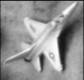
\includegraphics[width=\linewidth]{fig1_a}\vspace{2pt}
      
\includegraphics[width=\linewidth]{fig1_b}
       \end{minipage}
  }
  \subfloat[]{
    \begin{minipage}[b]{0.67\linewidth} 
      \centering
      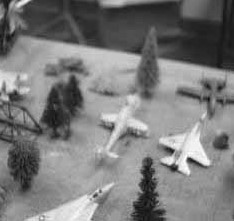
\includegraphics[width=\linewidth]{fig1_c}
       \end{minipage}
  }
  \end{minipage}
  \vfill
  \caption{本文实验所使用的模板图像和场景图像:(a) 模版图像, (b) 场景图像.}
  \label{fig:data}
\end{figure}


\subsection{相关匹配方法}

一般而言,欧式距离是最容易想到的相似性度量函数。对于给定的模版图像 M 和场景图像 N,其大小分别为 $m \times m$ 和 $n \times n\;(m>n)$,其欧式距离定义如下:

\begin{equation}
SSD=\sum_{i=1}^n \sum_{j=1}^n\left[M(i, j)-N(i, j)\right]^2
\vspace{0.5cm}
\end{equation}

将其展开可得:

\begin{equation}
\begin{split}
	SSD&=\sum_{i=1}^n \sum_{j=1}^n\left[M(i, j)\right]^2-2\sum_{i=1}^n \sum_{j=1}^n M(i, j)\cdot N(i, j)\\[0.5em]&+\sum_{i=1}^n \sum_{j=1}^n\left[N(i, j)\right]^2
\end{split}
\vspace{0.5cm}
\end{equation}

可以看出,只有第二项是有意义的,因为第一项和第三项的值在模板图像和窗口选定后是固定的。对于欧式距离而言,其值越大代表二者越不相似,即第二项的值越小则越不相似。将第二项进行归一化,可以得到相关度量的计算公式,如下:

\begin{equation}
C=\frac{\sum_{i=1}^n \sum_{j=1}^n M(i, j) N(i, j)}{\left[\sum_{i=1}^n \sum_{j=1}^n M(i, j)^2 \sum_{i=1}^n \sum_{j=1}^n N(i, j)^2\right]^{1 / 2}}
\vspace{0.5cm}
\end{equation}

代码实现如下:

\vspace{0.3cm}
\lstinputlisting[language=Python,firstline=43,lastline=45]{main.py}

对于相关匹配而言,为了更加准确地计算模板图像与场景图像的相关度量,还需要分别对二者进行归一化处理,代码如下:

\vspace{0.3cm}
\lstinputlisting[language=Python,firstline=81,lastline=108]{main.py}

\subsection{Hausdorff 距离匹配方法}

Hausdorff 距离是描述两组点之间相似程度的一种度量,它是集合和集合之间距离的一种定义形式。给定集合 $A=\{a_1,a_2,a_3,\cdots,a_n\}$ 和集合 $B=\{b_1,b_2,b_3,\cdots,b_n\}$,Hausdorff 距离的计算公式为:

\begin{equation}
h(A, B)=\max _{a \in A}\left\{\min _{b \in B}\{d(a, b)\}\right\}
\end{equation}

\begin{equation}
H(A, B)=\max \{h(A, B), h(B, A)\}
\vspace{0.5cm}
\end{equation}

$h(A, B)$ 即在计算出集合 $A$ 中每个点 $a_i$ 与集合 $B$ 中相距最近的点 $b_i$ 的距离的基础上,选出其中的最大值作为 $h(A, B)$ 的值。

代码实现如下:

\vspace{0.3cm}
\lstinputlisting[language=Python,firstline=48,lastline=52]{main.py}

Hausdorff 距离匹配方法的代码实现如下:

\vspace{0.3cm}
\lstinputlisting[language=Python,firstline=111,lastline=139]{main.py}

\subsection{图像距离变换方法}

图像距离变换主要是针对场景图像进行处理,在提取场景图像边缘的基础上,计算图像矩阵每个位置到提取的边缘最近的切比雪夫距离,从而得到距离矩阵,其计算公式如下:

\begin{equation}
\mathrm{DT}(p)=\min \{\mathrm{d}(\mathrm{p}, \mathrm{q})\} \text { with } \mathrm{q} \in \mathrm{B}
\end{equation}

\begin{equation}
d(p,q)=|i-x|+|j-y|
\vspace{0.5cm}
\end{equation}

其中,$p$ 为图像 $P$ 中的点,$B$ 是由 $P$ 的边缘点 $q$ 构成的集合,$(i,j)$ 和 $(x,y)$ 分别为 $p$ 和 $q$ 的坐标。

代码实现为:

\vspace{0.3cm}
\lstinputlisting[language=Python,firstline=55,lastline=64]{main.py}

经过提前计算得到图像矩阵每个位置的变换距离后,在模版匹配的过程中,只需要在距离矩阵中进行查找即可很快计算得到相似性度量,代码实现如下:

\vspace{0.3cm}
\lstinputlisting[language=Python,firstline=142,lastline=170]{main.py}